\section{Implementation}
The proposed scheme was implemented in Java as a library using Java Pairing Based Cryptography \cite{jpbc} library. The demo application developed uses this library in to demonstrate the features of this library. This work available under LGPL at anon-encrypt project hosted in google code \cite{ae}. All the functionality explained here carries unit tests (including application level functionality) and are integrated into the build.

\subsection{Library}

The output generated by various components in the library are encoded as XML. Basically certain classes can be serialized to produce the output to be used in as communication payload which is XML. Next we describe main components of the library and their implementation. All classes of the library are contained in $edu.purdue.cs626.anonencrypt$ package.\\

\subsubsection{Parameter Generator}
This is implemented in the $AEParameterGenerator$ class and will generate a new set of 2 level HIBE parameters to be used in setting up a peer. An example set of parameters are shown below (in the format used to publish the parameters.)

\lstinputlisting{xml/params.xml}

Contents of the XML elements G, G1, G2, G3, H1, H2 are base 64 encoded, binary representation of elements of group $\mathbb{G}$. \footnote{An element of group $\mathbb{G}$ is an elliptic cure element which is of the form (for example) \{x=28706359947801324, y=31910506035212, infFlag=0\}}\\

\subsubsection{Peer Key Generator}
Peer key generator is used to create private keys for contacts by a peer and is implemented in $RootKeyGen$. This generates an instance of $AEPrivateKey$ which can be serialized to obtain the certificate that contains the public parameters of the peer, if identifier and the private key created for the contact. A serialized instance of a private key is shown below:

\lstinputlisting{xml/privkey.xml}


\subsubsection{Contact key generator}
A contact of a peer instantiates $ContactKeyGen$ class with the private parameters provided by the peer and calls $getTmpPrivKey()$ with a random identifier to obtain the temporary key to decrypt information encrypted using the public identifier that it creates using the given random identifier.\\

\subsubsection{Cipher Implementation}
The modified HIBE encryption and decryption functions are implemented in $Encrypt$ and $Decrypt$. The cipher is implemented as a block cipher which encrypts an array of elements ($\in \mathbb{G}_1$) and outputs an instance of $AECipherText$ which includes the corresponding instances of $AECipherTextBlock$. The cipher text will be serialized using the $serialize()$ methods which produces an XML output. The decryptor will instantiate an $AECipherTextBlock$ instance using the serialized cipher text and will be able to decrypt each element and return the plain elements using the given private key. An example of serialized cipher text is shown below:\\

\subsubsection{Text Encoder}
It is important to note that the cipher implementation works on elements of the group $\mathbb{G}_1$. Therefore we need functions that encodes and decodes plain text to and from this group elements.
\begin{center}
$encode : {\{0,1\}}^* \rightarrow \mathbb{G}_1$\\
$decode : \mathbb{G}_1 \rightarrow {\{0,1\}}^*$\\
\end{center}

$TextEncoder$ class supports both these functionalities and is initialized with the public parameters. The $encode()$ method returns an array of elements $\in \mathbb{G}_1$ given a string value and the $decode()$ method return a byte array which is used to construct a string value, given an array of elements. \\

\subsubsection{Re-key}
The functionality required to re-key a peer is encapsulated in the $ReKey$ class. This is initialized with the current parameters and $update()$ function creates the new master key and $g_1$. Then an instance of $ReKeyInformation$ is created with a map of given $<I_{r_i}, r>$ values of the contacts. This is the information to publish, and an example (with two contacts) is shown below:

\lstinputlisting{xml/rekey.xml}

\subsection{Application}

Next we discuss the details of the application developed using the above library. This application uses a database with one simple table to hold all information of a contact such as contact's parameters, private key assigned to the peer by the contact, common name for the contact. Apache Derby \cite{derby} was used as the DBMS and the database instance is maintained in a configuration directory (called $.ae$) in the user home directory. Classes related to the application are included in the $edu.purdue.cs626.anonencrypt.app$ package.\\

\subsubsection{Update Request}
The $UpdateRequest$ class is used by a contact to generate a request to obtain the latest update of a peer. Given the name of a peer and a random identifier this generates the $ID_{req} = {h_1}^{I_{r_1}} \cdot {h_2}^{I_{r_2}}$ value and outputs the request as shown below:

\lstinputlisting{xml/req.xml}

\subsubsection{Update Response}
When a contact publishes a request for an $update$ another contact of the peer will be able to respond to this request and generate a response with the message from the peer. The contact that responds, can simply encrypt the message using the parameters of the peer after encoding the message to element of the group $\mathbb{G}_1$. The $UpdateResponse$ is used to generate the response message which if of the form:

\lstinputlisting{xml/resp.xml}

\subsubsection{Demo Application}
To demonstrate these capabilities a simple demo application was developed which displayed the set of options to install, add contacts and carry out operations with contacts. The message exchanges was demonstrated using a pop-up dialog displayed using Zenity\cite{zenity}.

\begin{center}
\begin{figure}[here]
\resizebox{!}{4.5cm}{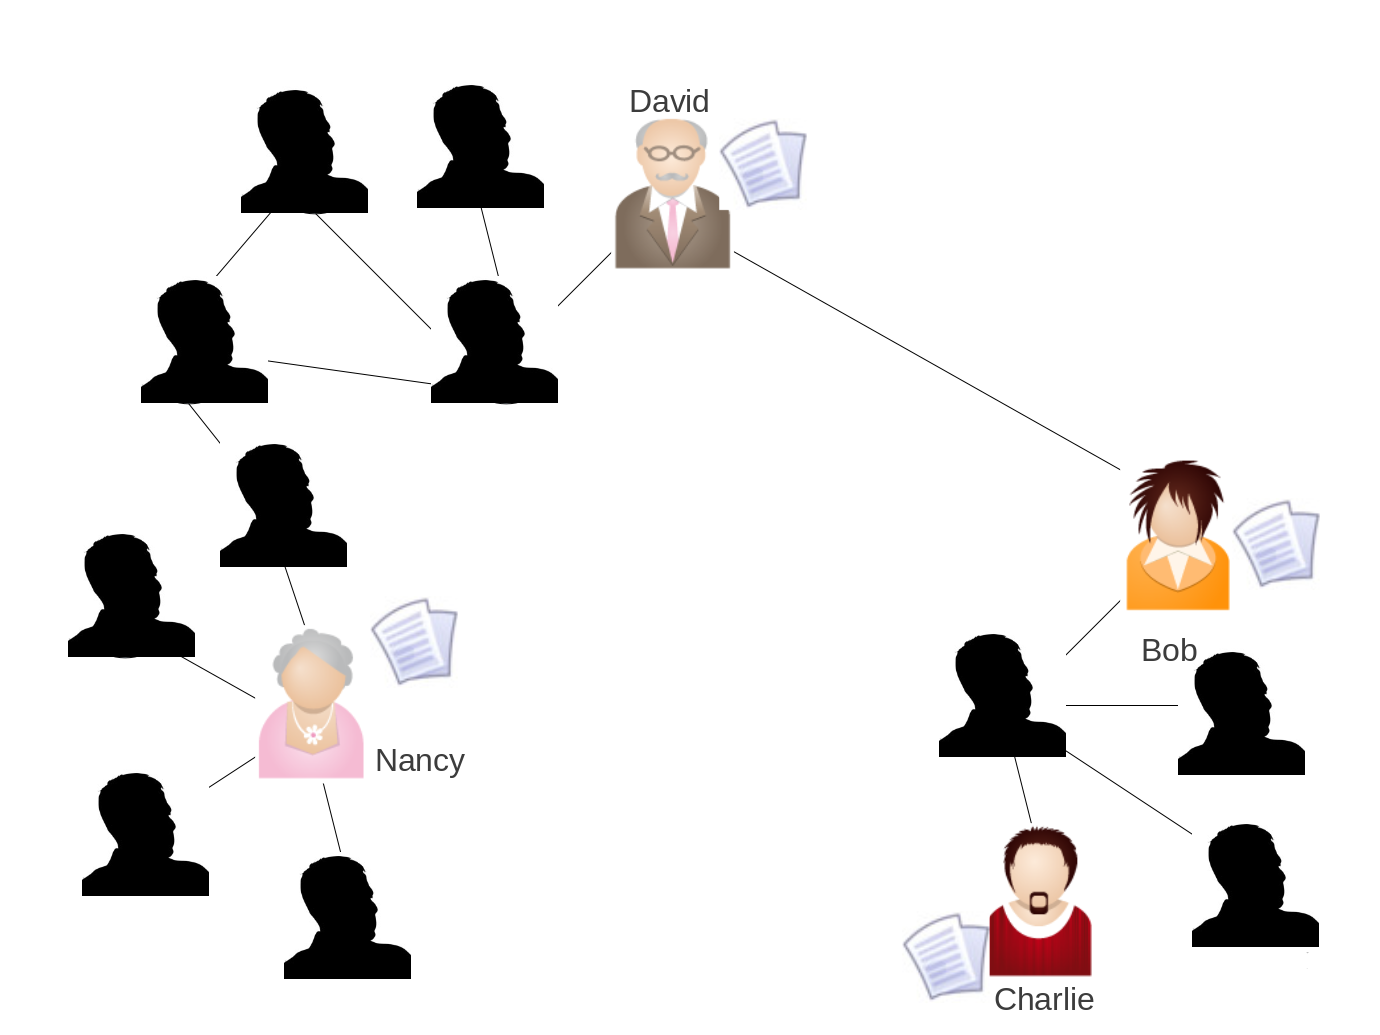
\includegraphics{img/img2.png}}
\caption{A screenshot of the demo application}
\label{fig:fig2}
\end{figure}
\end{center}
